\documentclass[aspectratio=169,11pt]{ctexbeamer}

\usetheme{Madrid}
\usecolortheme{default}

\usepackage{amsmath,amssymb,mathtools}
\usepackage{bm}
\usepackage{graphicx}

\makeatletter
\def\input@path{{../模板/}}
\makeatother
\usepackage{yingxing-beamer}

\title{凸函数}
\subtitle{定义、Jensen 不等式与导数判别}
\author{王晨旭}
\date{}

\newcommand{\R}{\mathbb{R}}
\newcommand{\abs}[1]{\left|#1\right|}
\newcommand{\dd}{\,\mathrm{d}}

\begin{document}

\begin{frame}
  \titlepage
\end{frame}

\begin{frame}{本讲目标}
\begin{itemize}
  \item 从割线几何理解凸函数：图像在弦线下方。
  \item 掌握凸函数的三种常用判别：割线斜率、Jensen 不等式、导数单调性。
  \item 会用凸性证明均值不等式、Young 不等式和幂函数不等式。
  \item 理解凸函数的连续性、可导性和切线支撑性质。
\end{itemize}
\end{frame}

\begin{frame}{二阶导数与弦线}
\small
设 $f$ 在 $[a,b]$ 上二阶可导，令 $l(x)$ 为连接两端点
$(a,f(a))$、$(b,f(b))$ 的线性函数：
\[
  l(x)=\frac{f(b)-f(a)}{b-a}(x-a)+f(a)
      =f(b)-\frac{f(b)-f(a)}{b-a}(b-x).
\]

由 Taylor 余项或插值余项可得，对某个 $\xi\in(a,b)$，
\[
  f(x)-l(x)=\frac12 f''(\xi)(x-a)(x-b).
\]

\begin{block}{直观结论}
若 $f''\ge 0$，则 $(x-a)(x-b)\le 0$，所以
\[
  f(x)\le l(x),\qquad x\in(a,b).
\]
也就是说，曲线位于任意弦线的下方。
\end{block}
\end{frame}

\begin{frame}{定义：凸函数}
\small
\begin{block}{定义 1}
设 $f$ 为区间 $I$ 上的函数。若对任意 $a<b$，$a,b\in I$，
任意 $x\in(a,b)$，都有
\[
  f(x)\le l(x),
\]
其中 $l(x)$ 是满足 $l(a)=f(a)$、$l(b)=f(b)$ 的线性函数，则称
$f$ 为 $I$ 上的\textbf{凸函数}。
\end{block}

\begin{itemize}
  \item 若不等号反向，则称 $f$ 为\textbf{凹函数}。
  \item 若对任意内部点都有严格不等式，则称 $f$ 为\textbf{严格凸函数}。
  \item 有时也把凸函数称为下凸函数，把凹函数称为上凸函数。
\end{itemize}
\end{frame}

\begin{frame}{先把方向记清楚}
\small
凸函数最容易混的是“不等号方向”。可以用下面三句话统一记忆。

\begin{block}{三种读法}
\begin{itemize}
  \item \textbf{几何读法：}两点之间的弦线在图像上方。
  \item \textbf{代数读法：}中间点的函数值不超过端点函数值的加权平均。
  \[
    f\bigl(ta+(1-t)b\bigr)\le t f(a)+(1-t)f(b).
  \]
  \item \textbf{导数读法：}若可导，斜率越来越大；若二阶可导，就是 $f''\ge0$。
\end{itemize}
\end{block}

凹函数的所有不等号方向都反过来。后面遇到 Jensen 不等式时，也按这个规则判断方向。
\end{frame}

\begin{frame}{几何图像}
\begin{center}
  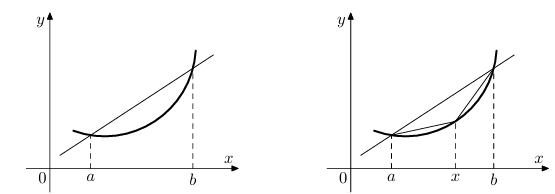
\includegraphics[width=0.72\linewidth]{assets/fig-5-5-convex-function.png}

  {\scriptsize 图 1\quad 凸函数}
\end{center}
\end{frame}

\begin{frame}{割线斜率判别}
\small
由 $f(x)\le l(x)$ 可改写为
\[
  \frac{f(x)-f(a)}{x-a}
  \le
  \frac{f(b)-f(a)}{b-a}
  \le
  \frac{f(b)-f(x)}{b-x},
  \qquad x\in(a,b).
\]

因此也有等价形式
\[
  \frac{f(x)-f(a)}{x-a}
  \le
  \frac{f(b)-f(x)}{b-x},
  \qquad x\in(a,b).
\]

\begin{block}{读法}
凸函数的割线斜率随区间右移而不减：左段斜率 $\le$ 整段斜率 $\le$ 右段斜率。
\end{block}
\end{frame}

\begin{frame}{等价的两点 Jensen 形式}
\small
令
\[
  x=ta+(1-t)b,\qquad t=\frac{b-x}{b-a}\in[0,1].
\]
则弦线函数可写为
\[
  l(x)=t f(a)+(1-t)f(b).
\]

于是凸性等价于
\[
  f\bigl(ta+(1-t)b\bigr)
  \le t f(a)+(1-t)f(b),
  \qquad 0<t<1.
\]

\begin{block}{要点}
两点 Jensen 不等式是凸函数最常用的代数表达。
\end{block}
\end{frame}

\begin{frame}{使用 Jensen 的基本步骤}
\small
遇到不等式题时，不要先硬算，先问三个问题。

\begin{enumerate}
  \item \textbf{选函数：}题目中出现 $\ln$、指数、幂、倒数、$\arctan$，通常先看它的凹凸性。
  \item \textbf{选权重：}若有平均数，用相等权重；若有 $1/p+1/q=1$，常用权重 $1/p,1/q$。
  \item \textbf{选点：}让 Jensen 左边的
  \[
    f\!\left(\sum \lambda_i x_i\right)
  \]
  变成题目里最难处理的那一项。
\end{enumerate}

\begin{block}{判断方向}
凸函数给出“$\le$”，凹函数给出“$\ge$”。这一步先判断错，整道题方向就会反。
\end{block}
\end{frame}

\begin{frame}{一个初等等价引理}
\small
若 $k,l>0$ 且
\[
  \frac{m}{k}\le \frac{n}{l},
\]
则
\[
  \frac{m}{k}\le \frac{m+n}{k+l}\le \frac{n}{l}.
\]

\begin{block}{用于凸性的地方}
若已知
\[
  \frac{f(x)-f(a)}{x-a}
  \le
  \frac{f(b)-f(x)}{b-x},
\]
则把两边按区间长度加权平均，可推出
\[
  \frac{f(x)-f(a)}{x-a}
  \le
  \frac{f(b)-f(a)}{b-a}
  \le
  \frac{f(b)-f(x)}{b-x}.
\]
\end{block}
\end{frame}

\begin{frame}{例 1：Young 不等式}
\small
考虑指数函数 $f(x)=e^x$。因为
\[
  f''(x)=e^x>0,
\]
所以 $e^x$ 是严格凸函数。

设 $a,b>0$，$p,q>1$，且
\[
  \frac1p+\frac1q=1.
\]
这里的配法是：权重取 $\frac1p,\frac1q$，点取 $\ln a^p$ 与 $\ln b^q$。这样
\[
  \frac1p\ln a^p+\frac1q\ln b^q=\ln a+\ln b=\ln(ab).
\]
由 $e^x$ 的凸性，
\[
  e^{\frac1p\ln a^p+\frac1q\ln b^q}
  \le
  \frac1p e^{\ln a^p}+\frac1q e^{\ln b^q}.
\]

因此
\[
  ab\le \frac{a^p}{p}+\frac{b^q}{q}.
\]
\end{frame}

\begin{frame}{定理 1：Jensen 不等式}
\small
\begin{block}{定理}
设 $f$ 是区间 $I$ 上的凸函数。若
\[
  x_i\in I,\quad \lambda_i\ge0\ (i=1,\dots,n),\quad
  \sum_{i=1}^n\lambda_i=1,
\]
则
\[
  f\!\left(\sum_{i=1}^n\lambda_i x_i\right)
  \le
  \sum_{i=1}^n \lambda_i f(x_i).
\]
\end{block}

\begin{itemize}
  \item $n=2$ 时就是两点 Jensen 形式。
  \item 一般情形可由数学归纳法推出。
\end{itemize}
\end{frame}

\begin{frame}{Jensen 不等式的归纳证明：合并权重}
\small
假设结论对 $n=k$ 已成立。对 $n=k+1$，不妨设
$0<\lambda_{k+1}<1$，于是
\[
  \sum_{i=1}^{k}\frac{\lambda_i}{1-\lambda_{k+1}}=1.
\]

这一步的意思是：先把前 $k$ 个点合成一个点
\[
  y=\sum_{i=1}^{k}\frac{\lambda_i}{1-\lambda_{k+1}}x_i,
\]
其中新的权重
\[
  \frac{\lambda_1}{1-\lambda_{k+1}},\dots,
  \frac{\lambda_k}{1-\lambda_{k+1}}
\]
之和为 $1$，所以可以对这 $k$ 个点使用归纳假设。
\end{frame}

\begin{frame}{Jensen 不等式的归纳证明：使用两点凸性}
\small
由
\[
  \sum_{i=1}^{k+1}\lambda_i x_i
  =(1-\lambda_{k+1})y+\lambda_{k+1}x_{k+1}
\]
可知，只需对 $y$ 与 $x_{k+1}$ 用两点凸性，再对 $y$ 用归纳假设：
\[
\begin{aligned}
f\!\left(\sum_{i=1}^{k+1}\lambda_i x_i\right)
&=f\!\left((1-\lambda_{k+1})
 \sum_{i=1}^{k}\frac{\lambda_i}{1-\lambda_{k+1}}x_i
 +\lambda_{k+1}x_{k+1}\right)\\
&\le (1-\lambda_{k+1})
 f\!\left(\sum_{i=1}^{k}\frac{\lambda_i}{1-\lambda_{k+1}}x_i\right)
 +\lambda_{k+1}f(x_{k+1})\\
&\le \sum_{i=1}^{k+1}\lambda_i f(x_i).
\end{aligned}
\]
\end{frame}

\begin{frame}{例 2：算术--几何平均值不等式}
\small
考虑函数
\[
  f(x)=-\ln x,\qquad x>0.
\]
因为
\[
  f''(x)=\frac1{x^2}>0,
\]
所以 $f$ 是严格凸函数。

对 $a_i>0$ 应用 Jensen 不等式，权重全部取 $\frac1n$，点取 $a_1,\dots,a_n$：
\[
  -\ln\frac{a_1+\cdots+a_n}{n}
  \le
  -\frac1n\sum_{i=1}^n\ln a_i.
\]
整理得
\[
  (a_1a_2\cdots a_n)^{1/n}
  \le
  \frac{a_1+a_2+\cdots+a_n}{n}.
\]
\end{frame}

\begin{frame}{命题 1：连续性}
\small
\begin{block}{命题}
设 $f$ 是区间 $I$ 上的凸函数。如果 $[a,b]$ 是 $I$ 中不含端点的闭区间，
则 $f$ 在 $[a,b]$ 上是 Lipschitz 函数。特别地，凸函数在区间内部总是连续的。
\end{block}

\begin{center}
  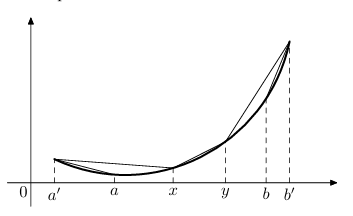
\includegraphics[width=0.45\linewidth]{assets/fig-5-6-continuity.png}

  {\scriptsize 图 2\quad 凸函数的连续性}
\end{center}
\end{frame}

\begin{frame}{连续性的证明思路}
\small
取 $a',b'\in I$，使
\[
  a'<a<b<b'.
\]
任取 $x<y$，$x,y\in[a,b]$。由凸函数的割线斜率单调性，
\[
\begin{aligned}
\frac{f(a')-f(a)}{a'-a}
&\le
\frac{f(a')-f(x)}{a'-x}
\le
\frac{f(y)-f(x)}{y-x}\\
&\le
\frac{f(b')-f(y)}{b'-y}
\le
\frac{f(b')-f(b)}{b'-b}.
\end{aligned}
\]

令
\[
  M=\max\left\{
  \left|\frac{f(a')-f(a)}{a'-a}\right|,
  \left|\frac{f(b')-f(b)}{b'-b}\right|
  \right\},
\]
则
\[
  |f(x)-f(y)|\le M|x-y|.
\]
\end{frame}

\begin{frame}{端点处可以不连续}
\small
凸函数在区间内部连续，但在区间端点处不一定连续。

\begin{block}{例}
定义在 $[0,+\infty)$ 上的函数
\[
  f(0)=1,\qquad f(x)=0\quad (x>0)
\]
是凸函数，但在 $x=0$ 处不连续。
\end{block}

\begin{itemize}
  \item 内点连续性来自局部 Lipschitz 性。
  \item 端点缺少左右两侧的割线控制，所以可以发生跳跃。
\end{itemize}
\end{frame}

\begin{frame}{命题 2：中点判别}
\small
\begin{block}{命题}
设 $f$ 是区间 $I$ 上的连续函数，则 $f$ 为凸函数当且仅当对任意
$x_1<x_2$，有
\[
  f\!\left(\frac{x_1+x_2}{2}\right)
  \le
  \frac12\bigl[f(x_1)+f(x_2)\bigr].
\]
\end{block}

\begin{itemize}
  \item 右侧称为\textbf{平均值不等式}或中点凸性。
  \item 若不要求连续，中点凸性本身不足以排除病态函数。
\end{itemize}
\end{frame}

\begin{frame}{中点判别：从中点到任意比例}
\small
只需说明：连续函数如果满足中点凸性，就能推出任意比例的 Jensen 形式。

先由中点不等式反复二分，得到
\[
  f\!\left(\frac{k}{2^m}a+\left(1-\frac{k}{2^m}\right)b\right)
  \le
  \frac{k}{2^m}f(a)+\left(1-\frac{k}{2^m}\right)f(b),
\]
其中 $m\in\mathbb N$，$0\le k\le 2^m$。这些比例称为\textbf{二进制有理数}。

任意 $t\in[0,1]$ 都可以用一列二进制有理数 $t_m$ 逼近。由 $f$ 连续，
令 $t_m\to t$，就得到
\[
  f\bigl(ta+(1-t)b\bigr)
  \le t f(a)+(1-t)f(b).
\]
这正是凸性的两点 Jensen 形式。
\end{frame}

\begin{frame}{推论 1：凸函数无内部极大值}
\small
\begin{block}{推论}
设 $f$ 是区间 $I$ 上的凸函数。若 $f$ 在 $I$ 的内部有极大值点，
则 $f$ 在内部是常值函数。
\end{block}

\begin{proof}
凸函数在 $I$ 的内部连续，并满足中点不等式。若内点取得局部最大，
中点不等式迫使邻域内的两侧函数值与最大值相同；继续向外推进，
可得在相应区间内恒为常值。
\end{proof}
\end{frame}

\begin{frame}{例 3：再次证明 $-\ln x$ 的凸性}
\small
对 $x,y>0$，由
\[
  (\sqrt{x}-\sqrt{y})^2\ge0
\]
可得
\[
  \sqrt{xy}\le \frac{x+y}{2}.
\]
两边取对数：
\[
  \frac12(\ln x+\ln y)
  \le
  \ln\frac{x+y}{2}.
\]

等价于
\[
  -\ln\frac{x+y}{2}
  \le
  \frac12\bigl[-\ln x-\ln y\bigr].
\]
由中点判别，连续函数 $-\ln x$ 是凸函数。
\end{frame}

\begin{frame}{命题 3：导数存在性}
\small
\begin{block}{命题}
设 $f$ 是区间 $I$ 上的凸函数，$x$ 为 $I$ 的内点，则 $f$ 在 $x$ 处的
左导数和右导数都存在，并且
\[
  f'_-(x)\le f'_+(x).
\]
\end{block}

取 $x_1<x<x_2$，由割线斜率单调性，
\[
  \frac{f(x)-f(x_1)}{x-x_1}
  \le
  \frac{f(x_2)-f(x)}{x_2-x}.
\]
左边关于 $x_1$ 单调，右边关于 $x_2$ 单调，由此两侧极限存在。
\end{frame}

\begin{frame}{凸函数的可导性备注}
\small
\begin{columns}[T]
\begin{column}{0.58\linewidth}
\begin{itemize}
  \item 凸函数不一定可微。例如
  \[
    f(x)=|x|
  \]
  是凸函数，但在 $x=0$ 处不可微。
  \item 凸函数的不可微点至多可数。
  \item 对于可微函数，可以用导函数的单调性来判别凸性。
\end{itemize}
\end{column}

\begin{column}{0.36\linewidth}
\begin{center}
  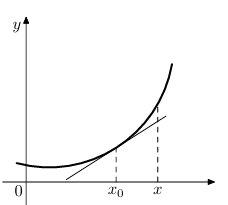
\includegraphics[width=0.9\linewidth]{assets/fig-5-7-differentiability.png}

  {\scriptsize 图 3\quad 凸函数的可微性}
\end{center}
\end{column}
\end{columns}
\end{frame}

\begin{frame}{命题 4：可微函数的凸性判别}
\small
\begin{block}{命题}
设 $f$ 是区间 $I$ 上的可微函数，则以下两条等价于 $f$ 为凸函数：
\begin{enumerate}
  \item $f'$ 为单调递增函数；
  \item 对任意 $x_0,x\in I$，有
  \[
    f(x)\ge f'(x_0)(x-x_0)+f(x_0).
  \]
\end{enumerate}
\end{block}

第二条说明：凸函数的图像位于任意切线的上方。
\end{frame}

\begin{frame}{导数判别的直观含义}
\small
可微时，凸性可以理解为“斜率越来越大”。

\begin{itemize}
  \item 若 $f'$ 递增，则从左到右切线越来越陡，图像只能向上弯。
  \item 切线支撑不等式
  \[
    f(x)\ge f(x_0)+f'(x_0)(x-x_0)
  \]
  表示：任取一点作切线，整条曲线都在这条切线的上方。
  \item 做题时，二阶可导优先算 $f''$；只有 $f''$ 不方便时，再用 Jensen 或割线斜率。
\end{itemize}
\end{frame}

\begin{frame}{导数判别：必要性}
\small
若 $f$ 是可微凸函数，任取 $x_1<x_2$。当 $x\in(x_1,x_2)$ 时，
\[
  \frac{f(x)-f(x_1)}{x-x_1}
  \le
  \frac{f(x_2)-f(x_1)}{x_2-x_1}
  \le
  \frac{f(x_2)-f(x)}{x_2-x}.
\]
令 $x\to x_1+$ 和 $x\to x_2-$，得
\[
  f'(x_1)
  \le
  \frac{f(x_2)-f(x_1)}{x_2-x_1}
  \le
  f'(x_2).
\]
所以 $f'$ 单调递增。
\end{frame}

\begin{frame}{导数判别：充分性}
\small
反过来，若 $f'$ 单调递增，任取 $a<x<b$。由微分中值定理，
存在
\[
  \xi_1\in(a,x),\qquad \xi_2\in(x,b),
\]
使
\[
  f(x)-f(a)=f'(\xi_1)(x-a),\qquad
  f(b)-f(x)=f'(\xi_2)(b-x).
\]

因为 $\xi_1<\xi_2$，所以
\[
  f'(\xi_1)\le f'(\xi_2),
\]
于是
\[
  \frac{f(x)-f(a)}{x-a}
  \le
  \frac{f(b)-f(x)}{b-x}.
\]
由割线判别可知 $f$ 为凸函数。
\end{frame}

\begin{frame}{切线支撑不等式}
\small
若 $f$ 可微且凸，取 $x_0\in I$。

当 $x>x_0$ 时，由割线斜率判别，
\[
  f'(x_0)\le \frac{f(x)-f(x_0)}{x-x_0}.
\]
当 $x<x_0$ 时，同理得到
\[
  \frac{f(x_0)-f(x)}{x_0-x}\le f'(x_0).
\]

两种情形合并为
\[
  f(x)\ge f'(x_0)(x-x_0)+f(x_0).
\]
\end{frame}

\begin{frame}{命题 5：二阶导数判别}
\small
\begin{block}{命题}
若 $f$ 在区间 $I$ 上二阶可导，则
\[
  f \text{ 为凸函数}\quad \Longleftrightarrow\quad f''(x)\ge0,\ \forall x\in I.
\]
\end{block}

\begin{proof}
由命题 4，$f$ 凸当且仅当 $f'$ 单调递增；而 $f'$ 单调递增当且仅当
其导数 $f''$ 非负。
\end{proof}
\end{frame}

\begin{frame}{例 4：幂函数不等式}
\small
设 $p\ge1$。当 $a,b\ge0$ 时，
\[
  \left(\frac{a+b}{2}\right)^p
  \le
  \frac{a^p+b^p}{2}.
\]

\begin{proof}
若 $a=0$ 或 $b=0$，结论显然。若 $a,b>0$，考虑
\[
  f(x)=x^p,\qquad x>0.
\]
因为
\[
  f''(x)=p(p-1)x^{p-2}\ge0,
\]
所以 $f$ 在 $(0,+\infty)$ 上为凸函数。由两点 Jensen 不等式得到结论。
\end{proof}
\end{frame}

\begin{frame}{例 5：距离函数的凸性}
\small
设 $P=(a,b)$ 为平面上的固定点。$x$ 轴上的点 $(x,0)$ 到 $P$ 的距离函数为
\[
  f(x)=\sqrt{(x-a)^2+b^2},\qquad x\in\R.
\]
若 $b\ne0$，则
\[
  f'(x)=\frac{x-a}{\sqrt{(x-a)^2+b^2}},
\]
\[
  f''(x)=
  \frac{1}{\sqrt{(x-a)^2+b^2}}
  -\frac{(x-a)^2}{\bigl[(x-a)^2+b^2\bigr]^{3/2}}
  =
  \frac{b^2}{\bigl[(x-a)^2+b^2\bigr]^{3/2}}>0.
\]
因此 $f$ 是凸函数。
\end{frame}

\begin{frame}{距离函数的几何解释}
\begin{columns}[T]
\begin{column}{0.52\linewidth}
\small
凸性给出
\[
  f\!\left(\frac{x+y}{2}\right)
  \le
  \frac12\bigl[f(x)+f(y)\bigr].
\]
几何上，这表示三角形中从顶点 $P$ 出发的中线长度不超过从 $P$ 出发的两边长度和的一半。
\end{column}
\begin{column}{0.43\linewidth}
\begin{center}
  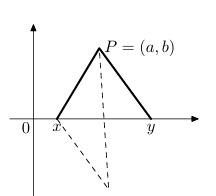
\includegraphics[width=0.9\linewidth]{assets/fig-5-8-distance-convexity.jpg}

  {\scriptsize 图 4\quad 距离函数的凸性}
\end{center}
\end{column}
\end{columns}
\end{frame}

\begin{frame}{习题与解答}
\begin{itemize}
  \item 本节习题主要训练三类方法：二阶导数判别、Jensen 不等式、局部凸性。
  \item 每道题先单独给出题目，再单独给出解答，便于课堂停顿和学生先做。
  \item 函数默认在题目给出的区间上讨论；未写区间时按自然定义域或整个 $\R$ 讨论。
\end{itemize}
\end{frame}

\begin{frame}{习题解题路线}
\small
拿到题目后，可以按下面顺序判断方法。

\begin{enumerate}
  \item \textbf{要证明函数凸凹：}先看是否二阶可导，能算 $f''$ 就先算。
  \item \textbf{要证明均值型不等式：}优先找凸函数或凹函数，然后套 Jensen。
  \item \textbf{题目含“局部”“极值”“有界”：}优先用凸函数的几何性质，例如无内部严格极大值、割线斜率单调。
\end{enumerate}

下面的解答会尽量写出“为什么选这个方法”，而不只写计算结果。
\end{frame}

\begin{frame}{练习 1：题目}
\small
\textbf{研究下列函数的凸凹性：}
\[
  (1)\ f(x)=x^p\ (x\ge0,\ 0<p\le1);
\]
\[
  (2)\ f(x)=a^x\ (a>0);
  \qquad
  (3)\ f(x)=x\ln x.
\]
\end{frame}

\begin{frame}{练习 1：解答}
\small
\begin{enumerate}
  \item 当 $0<p<1$ 时，
  \[
    f''(x)=p(p-1)x^{p-2}<0\qquad (x>0),
  \]
  故 $x^p$ 在 $(0,+\infty)$ 上严格凹，在 $[0,+\infty)$ 上凹；当 $p=1$ 时为线性函数。
  \item
  \[
    (a^x)''=(\ln a)^2a^x\ge0.
  \]
  若 $a\ne1$，则 $a^x$ 严格凸；若 $a=1$，则为常值函数。
  \item 在 $(0,+\infty)$ 上，
  \[
    (x\ln x)''=\frac1x>0,
  \]
  所以 $x\ln x$ 严格凸。若把它按极限补充定义为 $f(0)=0$，则它在
  $[0,+\infty)$ 上仍为凸函数。
\end{enumerate}
\end{frame}

\begin{frame}{练习 2：题目}
\small
\textbf{研究函数}
\[
  f(x)=\ln\frac{x}{\sin x}
\]
\textbf{在区间 $\left[0,\dfrac{\pi}{2}\right]$ 上的凸性。}
\end{frame}

\begin{frame}{练习 2：解答}
\small
在 $x=0$ 处按极限补充定义 $f(0)=0$。当 $0<x\le\dfrac{\pi}{2}$ 时，
\[
  f'(x)=\frac1x-\cot x,
\]
\[
  f''(x)=-\frac1{x^2}+\csc^2 x
  =\frac1{\sin^2 x}-\frac1{x^2}.
\]
由于 $0<\sin x\le x$，故
\[
  \frac1{\sin^2 x}\ge \frac1{x^2}.
\]
于是 $f''(x)\ge0$，且在 $(0,\pi/2]$ 上严格大于 $0$。再加上
$x\to0+$ 时 $f(x)\to0$，所以连续延拓到端点后，$f$ 在
$\left[0,\dfrac{\pi}{2}\right]$ 上为凸函数。
\end{frame}

\begin{frame}{练习 3：题目}
\small
\textbf{设 $f$ 在 $[a,b]$ 上连续，在 $(a,b)$ 中二阶可微，}
\[
  f(a)=f(b)=0,
\]
\textbf{并且存在 $c\in(a,b)$ 使得 $f(c)>0$。证明：存在
$\xi\in(a,b)$，使得}
\[
  f''(\xi)<0.
\]
\end{frame}

\begin{frame}{练习 3：解答}
\small
反设 $f''(x)\ge0$ 对一切 $x\in(a,b)$ 成立。则 $f$ 在 $[a,b]$ 上为凸函数。

连接端点的弦线恒为 $0$，由凸函数位于弦线下方可得
\[
  f(x)\le0,\qquad x\in[a,b].
\]
这与 $f(c)>0$ 矛盾。因此 $f''$ 不可能处处非负，故存在
$\xi\in(a,b)$ 使
\[
  f''(\xi)<0.
\]
\end{frame}

\begin{frame}{练习 4：题目}
\small
\textbf{证明：如果 $f,g$ 均为区间 $I$ 中的凸函数，则}
\[
  h(x)=\max\{f(x),g(x)\}
\]
\textbf{也是 $I$ 中的凸函数。}
\end{frame}

\begin{frame}{练习 4：解答}
\small
任取 $x,y\in I$ 和 $\lambda\in[0,1]$。由 $f,g$ 的凸性，
\[
\begin{aligned}
h(\lambda x+(1-\lambda)y)
&=\max\{f(\lambda x+(1-\lambda)y),g(\lambda x+(1-\lambda)y)\}\\
&\le \max\{\lambda f(x)+(1-\lambda)f(y),
           \lambda g(x)+(1-\lambda)g(y)\}.
\end{aligned}
\]
又因为
\[
  f(x),g(x)\le h(x),\qquad f(y),g(y)\le h(y),
\]
所以
\[
  h(\lambda x+(1-\lambda)y)
  \le \lambda h(x)+(1-\lambda)h(y).
\]
故 $h$ 为凸函数。
\end{frame}

\begin{frame}{练习 5：题目}
\small
\textbf{设函数 $f(x)$ 和 $g(x)$ 均为凸函数，且 $f$ 单调递增。证明：}
\[
  f(g(x))
\]
\textbf{也是凸函数。}
\end{frame}

\begin{frame}{练习 5：解答}
\small
默认 $g$ 的值域落在 $f$ 的定义域内。复合题的关键是两步：先用 $g$ 的凸性，
再用 $f$ 的单调性保持不等号方向。

设 $x,y$ 在 $g$ 的定义区间内，$\lambda\in[0,1]$。由 $g$ 的凸性，
\[
  g(\lambda x+(1-\lambda)y)
  \le
  \lambda g(x)+(1-\lambda)g(y).
\]
由于 $f$ 单调递增，
\[
  f(g(\lambda x+(1-\lambda)y))
  \le
  f(\lambda g(x)+(1-\lambda)g(y)).
\]
再由 $f$ 的凸性，
\[
  f(\lambda g(x)+(1-\lambda)g(y))
  \le
  \lambda f(g(x))+(1-\lambda)f(g(y)).
\]
故 $f\circ g$ 为凸函数。
\end{frame}

\begin{frame}{练习 6：题目}
\small
\textbf{证明三次的实系数多项式不是凸函数。}

\vspace{1em}
这里的意思是：作为定义在整个 $\R$ 上的函数，它不可能是凸函数；若只看某个较小区间，
三次函数有可能在该区间上凸。
\end{frame}

\begin{frame}{练习 6：解答}
\small
设
\[
  P(x)=ax^3+bx^2+cx+d,\qquad a\ne0.
\]
则
\[
  P''(x)=6ax+2b.
\]
由于 $a\ne0$，$P''(x)$ 是一次函数，它在整个 $\R$ 上必然变号：
\[
  x\to+\infty \quad\text{和}\quad x\to-\infty
\]
时，$6ax+2b$ 的符号相反。

若 $P$ 在整个 $\R$ 上为凸函数，则应有 $P''(x)\ge0$ 对一切 $x\in\R$
成立，这与上面的变号矛盾。因此三次实系数多项式在整个 $\R$ 上不是凸函数。
\end{frame}

\begin{frame}{练习 7：题目}
\small
\textbf{设 $a,b\ge0$，证明}
\[
  2\arctan\frac{a+b}{2}\ge \arctan a+\arctan b.
\]
\end{frame}

\begin{frame}{练习 7：解答}
\small
令
\[
  \varphi(x)=\arctan x,\qquad x\ge0.
\]
则
\[
  \varphi''(x)= -\frac{2x}{(1+x^2)^2}\le0.
\]
所以 $\varphi$ 在 $[0,+\infty)$ 上为凹函数。由凹函数的 Jensen 不等式，
\[
  \varphi\!\left(\frac{a+b}{2}\right)
  \ge
  \frac{\varphi(a)+\varphi(b)}{2}.
\]
代回 $\varphi(x)=\arctan x$ 即得
\[
  2\arctan\frac{a+b}{2}\ge \arctan a+\arctan b.
\]
等号当且仅当 $a=b$。
\end{frame}

\begin{frame}{练习 8：题目}
\small
\textbf{设 $a_i>0\ (1\le i\le n)$，证明}
\[
  \frac{n}{\dfrac1{a_1}+\dfrac1{a_2}+\cdots+\dfrac1{a_n}}
  \le
  \sqrt[n]{a_1a_2\cdots a_n}.
\]
\end{frame}

\begin{frame}{练习 8：解答}
\small
对正数
\[
  b_i=\frac1{a_i}
\]
应用算术--几何平均值不等式，得到
\[
  \frac{\dfrac1{a_1}+\cdots+\dfrac1{a_n}}{n}
  \ge
  \sqrt[n]{\frac1{a_1a_2\cdots a_n}}
  =
  \frac1{\sqrt[n]{a_1a_2\cdots a_n}}.
\]
两边取倒数即得结论。等号当且仅当
\[
  a_1=a_2=\cdots=a_n.
\]
\end{frame}

\begin{frame}{练习 9：题目}
\small
\textbf{设 $a_i>0\ (1\le i\le n)$，且}
\[
  \sum_{i=1}^n a_i=1.
\]
\textbf{证明对任意 $x_i\ge0$，}
\[
  x_1^{a_1}x_2^{a_2}\cdots x_n^{a_n}
  \le
  \sum_{i=1}^n a_i x_i,
\]
\textbf{并求等号成立的条件。}
\end{frame}

\begin{frame}{练习 9：解答}
\small
若某个 $x_i=0$ 而不是所有 $x_i$ 都为 $0$，则左边为 $0$，右边为正，
不等式严格成立。若所有 $x_i=0$，等号成立。

下面设 $x_i>0$。由于 $\ln x$ 是凹函数，由 Jensen 不等式，
\[
  \sum_{i=1}^n a_i\ln x_i
  \le
  \ln\left(\sum_{i=1}^n a_i x_i\right).
\]
两边取指数，得
\[
  \prod_{i=1}^n x_i^{a_i}
  \le
  \sum_{i=1}^n a_i x_i.
\]
结合前面的零值情形，等号当且仅当
\[
  x_1=x_2=\cdots=x_n.
\]
\end{frame}

\begin{frame}{练习 10：题目}
\small
\textbf{设 $f$ 为区间 $I$ 中的凸函数，$x_0$ 为 $I$ 的内点。如果 $x_0$ 为
$f$ 的极值点，则证明：}
\[
  f \text{ 在 } x_0 \text{ 的左边单调递减，}
\]
\[
  f \text{ 在 } x_0 \text{ 的右边单调递增。}
\]
\end{frame}

\begin{frame}{练习 10：解答思路}
\small
先处理“极大”的可能性。若 $x_0$ 是局部极大点，取 $u<x_0<v$ 且足够靠近
$x_0$，使得
\[
  f(u)\le f(x_0),\qquad f(v)\le f(x_0).
\]
由凸性，$f(x_0)$ 又不超过 $f(u)$ 与 $f(v)$ 的加权平均，于是三者只能相等。
所以凸函数的内点局部极大只能落在一段平坦区间上，也可看成局部极小点。

下面设 $x_0$ 是局部极小点。若存在 $y>x_0$ 使 $f(y)<f(x_0)$，则对充分小的
$t>0$，
\[
  x_t=(1-t)x_0+ty
\]
仍在 $x_0$ 的极小邻域内，但凸性给出
\[
  f(x_t)\le (1-t)f(x_0)+t f(y)<f(x_0),
\]
矛盾。左侧同理。所以 $x_0$ 是全局极小点。
\end{frame}

\begin{frame}{练习 10：证明}
\small
由上一页可知
\[
  f(x)\ge f(x_0),\qquad x\in I.
\]
任取 $x_1<x_2<x_0$。因为 $x_2$ 位于 $x_1$ 与 $x_0$ 之间，存在
$\lambda\in(0,1)$ 使
\[
  x_2=\lambda x_1+(1-\lambda)x_0.
\]
由凸性和 $f(x_0)\le f(x_2)$，
\[
  f(x_2)\le \lambda f(x_1)+(1-\lambda)f(x_0)
  \le \lambda f(x_1)+(1-\lambda)f(x_2).
\]
整理得 $f(x_2)\le f(x_1)$，故 $f$ 在 $x_0$ 左边单调递减。

同理，若 $x_0<x_1<x_2$，则
\[
  x_1=\lambda x_0+(1-\lambda)x_2,
\]
由凸性可得 $f(x_1)\le f(x_2)$，故 $f$ 在 $x_0$ 右边单调递增。
\end{frame}

\begin{frame}{练习 11：题目}
\small
\textbf{证明：定义在整个 $\R$ 上的有界凸函数必为常值函数。}
\end{frame}

\begin{frame}{练习 11：解答}
\small
反设 $f$ 不是常值函数，则存在 $x_1<x_2$ 使
\[
  f(x_1)\ne f(x_2).
\]
若 $f(x_2)>f(x_1)$，记
\[
  m=\frac{f(x_2)-f(x_1)}{x_2-x_1}>0.
\]
由凸函数割线斜率的单调性，对任意 $x>x_2$ 有
\[
  \frac{f(x)-f(x_1)}{x-x_1}\ge m,
\]
从而
\[
  f(x)\ge f(x_1)+m(x-x_1)\to+\infty.
\]
这与有界性矛盾。

若 $f(x_2)<f(x_1)$，同理令 $x\to-\infty$ 也得到矛盾。因此 $f$ 必为常值函数。
\end{frame}

\begin{frame}{练习 12：题目}
\small
\textbf{设 $f(x)$ 是定义在区间 $I$ 中的连续函数。如果任给 $x_0\in I$，
均存在 $\delta>0$，使得 $f(x)$ 在区间}
\[
  I\cap(x_0-\delta,x_0+\delta)
\]
\textbf{中是凸函数，则证明 $f(x)$ 是 $I$ 中的凸函数。}
\end{frame}

\begin{frame}{练习 12：解答思路}
\small
任取 $a<b$，$a,b\in I$，令 $l(x)$ 为连接 $(a,f(a))$ 与 $(b,f(b))$
的线性函数，并设
\[
  g(x)=f(x)-l(x).
\]
则 $g$ 连续、局部凸，且
\[
  g(a)=g(b)=0.
\]
只需证明
\[
  g(x)\le0,\qquad x\in[a,b].
\]
这一步的意思是：只要能证明 $f$ 在任意两点弦线下方，就得到整体凸性。
\end{frame}

\begin{frame}{练习 12：证明}
\small
反设 $g$ 在 $[a,b]$ 上有正最大值 $M>0$，并令
\[
  E=\{x\in(a,b)\mid g(x)=M\}.
\]
则 $E$ 非空且闭。

若 $x_0\in E$，由于 $g$ 在 $x_0$ 附近凸，且 $x_0$ 是局部最大点，
凸性迫使 $g$ 在 $x_0$ 的某个邻域内恒等于 $M$。具体地，对充分小的 $h$，
\[
  M=g(x_0)\le \frac{g(x_0-h)+g(x_0+h)}2\le M,
\]
所以 $g(x_0-h)=g(x_0+h)=M$。因此 $E$ 在 $(a,b)$ 中也是开集。

于是 $E$ 是连通区间 $(a,b)$ 中的非空既开又闭子集，只能有 $E=(a,b)$。
由连续性得到 $g(a)=g(b)=M$，与 $g(a)=g(b)=0$ 矛盾。
故 $g(x)\le0$，所以 $f$ 在 $I$ 上为凸函数。
\end{frame}

\begin{frame}{练习 13：题目}
\small
\textbf{设 $f$ 为 $(-\infty,+\infty)$ 中的连续函数，如果对任意
$x\in\R$，均有}
\[
  \lim_{h\to0}
  \frac{f(x+h)+f(x-h)-2f(x)}{h^2}=0,
\]
\textbf{证明 $f(x)$ 为线性函数。}
\end{frame}

\begin{frame}{练习 13：解答思路}
\small
任取 $\varepsilon>0$，令
\[
  F_\varepsilon(x)=f(x)+\varepsilon x^2.
\]
这样做的目的，是把“二阶对称差商等于 $0$”变成“严格为正”。直观上，
$F_\varepsilon$ 应该表现得像凸函数。

事实上，
\[
  \lim_{h\to0}
  \frac{F_\varepsilon(x+h)+F_\varepsilon(x-h)-2F_\varepsilon(x)}{h^2}
  =2\varepsilon>0.
\]
下面证明 $F_\varepsilon$ 是凸函数。
\end{frame}

\begin{frame}{练习 13：证明}
\small
若 $F_\varepsilon$ 不凸，则存在 $a<b$，使得 $F_\varepsilon$ 在 $[a,b]$
上某点高于连接两端点的弦线。令 $l$ 为该弦线，设
\[
  g(x)=F_\varepsilon(x)-l(x).
\]
则 $g(a)=g(b)=0$，且 $g$ 在某个 $x_0\in(a,b)$ 处取得正最大值。

对充分小的 $h$，
\[
  g(x_0+h)+g(x_0-h)-2g(x_0)\le0.
\]
这是因为 $g(x_0)$ 是附近最大的值，左右两点都不超过它。但线性函数的二阶对称差商为 $0$，
所以减去弦线不会改变二阶对称差商：
\[
\begin{aligned}
&\lim_{h\to0}
\frac{g(x_0+h)+g(x_0-h)-2g(x_0)}{h^2}\\
&\qquad =
\lim_{h\to0}
\frac{F_\varepsilon(x_0+h)+F_\varepsilon(x_0-h)-2F_\varepsilon(x_0)}{h^2}
=2\varepsilon>0,
\end{aligned}
\]
矛盾。因此 $F_\varepsilon$ 为凸函数。
\end{frame}

\begin{frame}{练习 13：证明（续）}
\small
于是对任意 $a,b\in\R$ 和 $t\in[0,1]$，
\[
  f(ta+(1-t)b)+\varepsilon(ta+(1-t)b)^2
  \le
  t[f(a)+\varepsilon a^2]+(1-t)[f(b)+\varepsilon b^2].
\]
令 $\varepsilon\to0+$，得到
\[
  f(ta+(1-t)b)\le t f(a)+(1-t)f(b),
\]
所以 $f$ 为凸函数。

同理，对
\[
  H_\varepsilon(x)=-f(x)+\varepsilon x^2
\]
重复上面的论证可知 $H_\varepsilon$ 为凸函数。令 $\varepsilon\to0+$，
得到 $-f$ 为凸函数，即 $f$ 为凹函数。

故 $f$ 既凸又凹。于是对任意 $a<b$，$f$ 在 $[a,b]$ 上等于连接端点的弦线，
所以 $f$ 为线性函数。
\end{frame}

\begin{frame}{课堂小结}
\begin{itemize}
  \item 凸函数的核心图像：任意弦线在图像上方。
  \item 常用判别链条：
  \[
    f''\ge0 \Rightarrow f'\ \text{递增}
    \Rightarrow \text{割线斜率递增}
    \Rightarrow \text{Jensen 不等式}.
  \]
  \item 连续凸函数可由中点不等式判别。
  \item 凸函数是证明不等式的重要工具：先找凸函数，再套 Jensen。
\end{itemize}
\end{frame}

\end{document}
